\documentclass{standalone}
\usepackage{tkz-fct}
\usepackage{tkz-euclide}
\usepackage{color}
\usepackage{amsmath}
\renewcommand*\familydefault{\sfdefault}
\usepackage{sansmath}
\sansmath
\definecolor{gray75}{gray}{0.75}
\begin{document}
 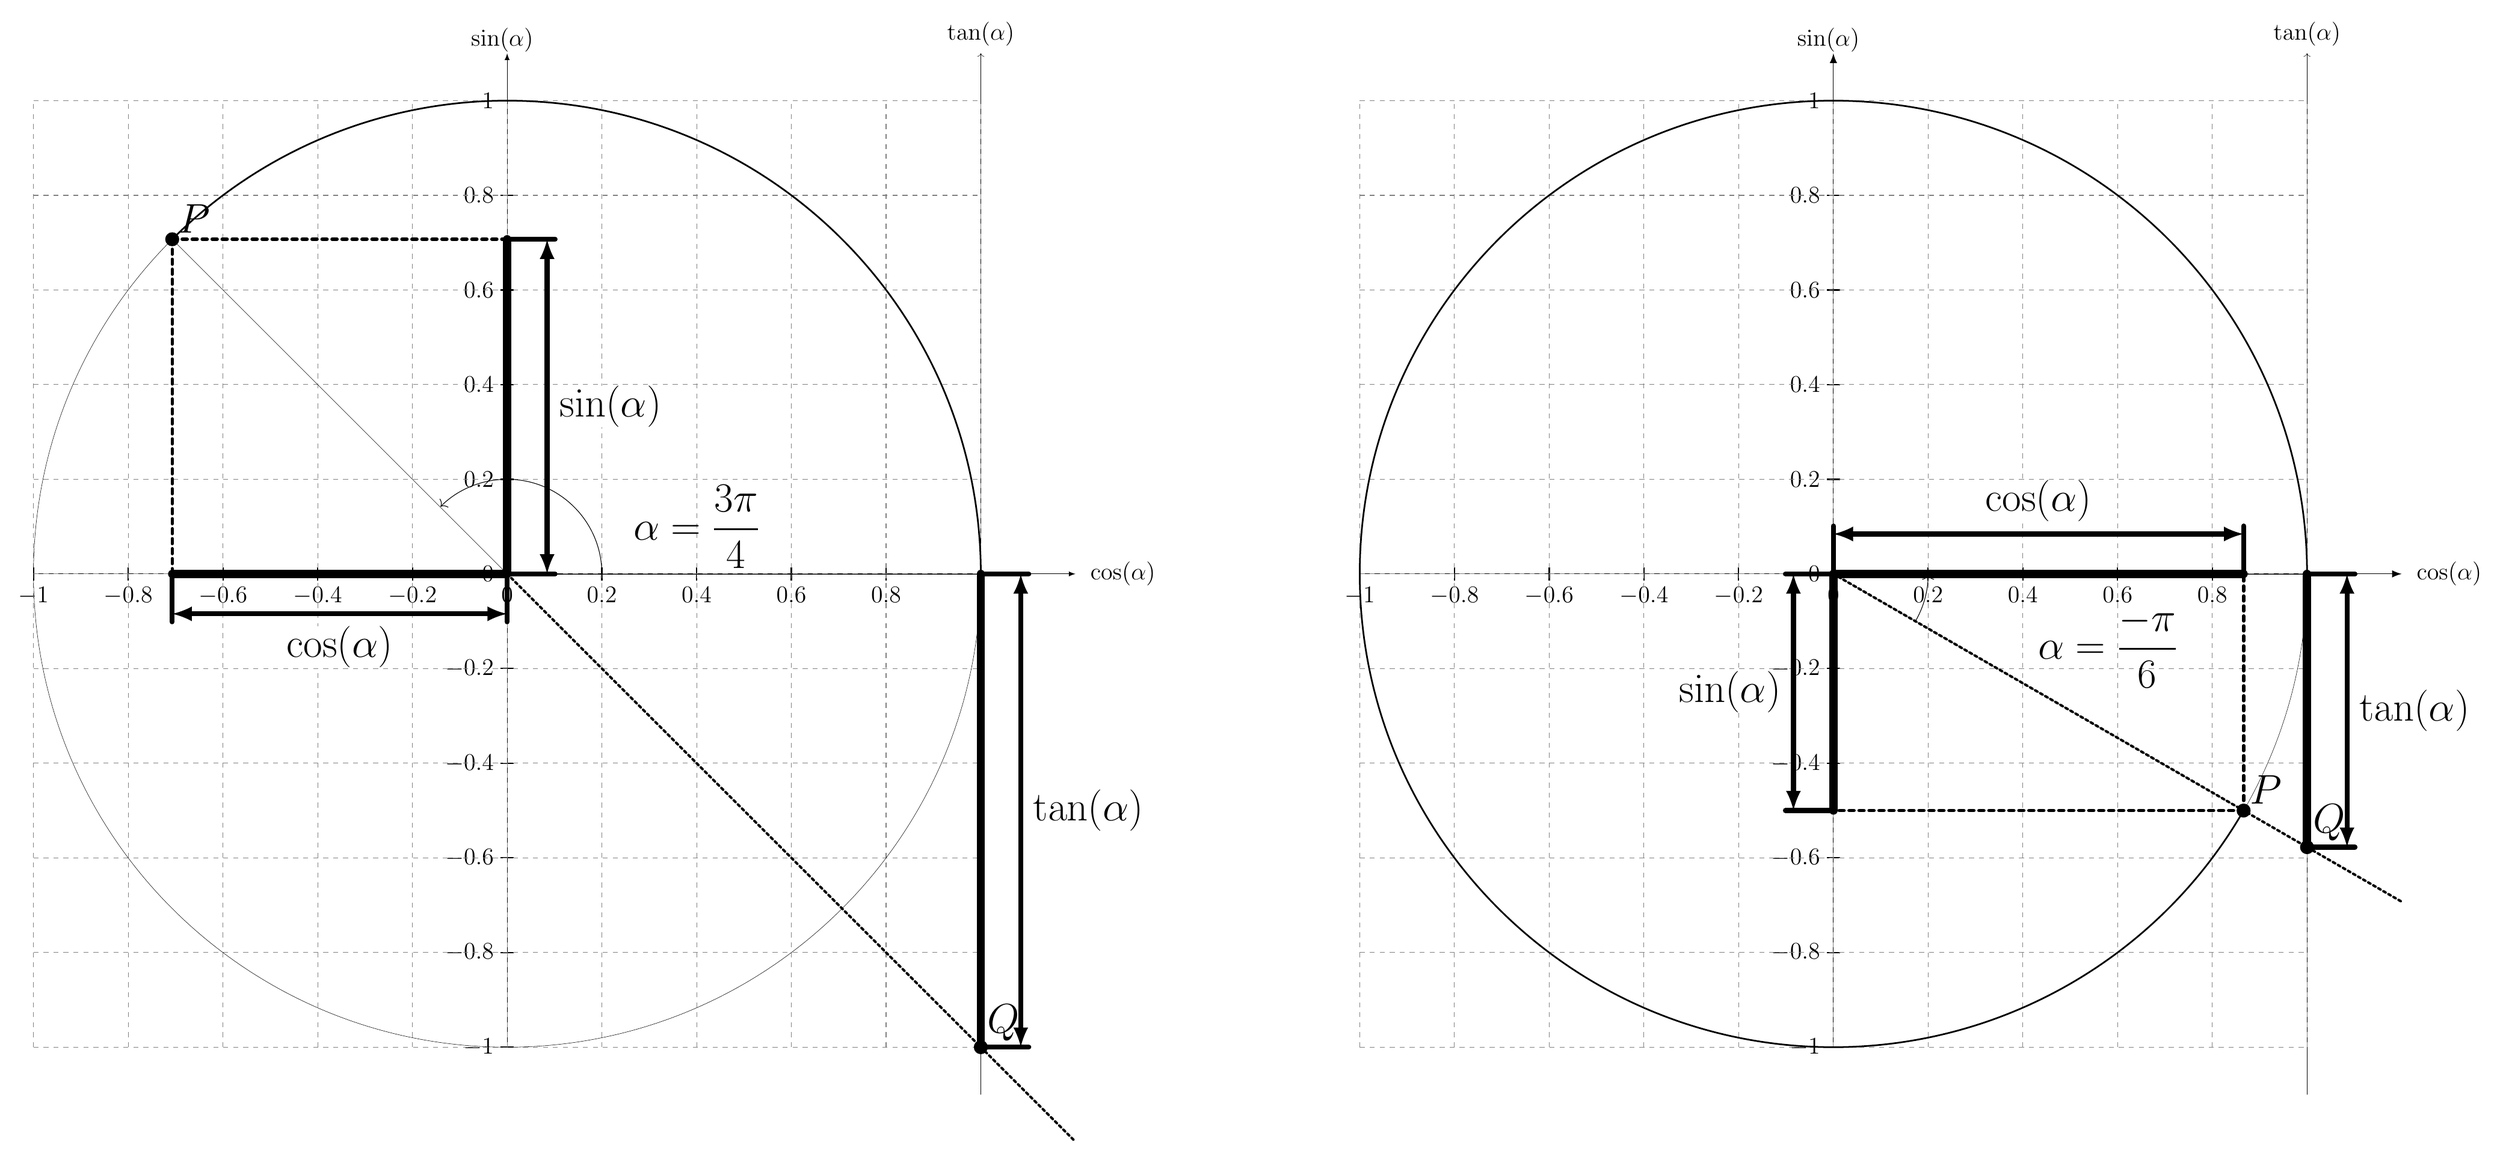
\begin{tikzpicture}[scale=2]
   \tkzInit[xmax=1.,ymax=1.,xmin=-1. ,ymin=-1,xstep=0.2,ystep=0.2]
   \tkzDrawY[label=$\sin(\alpha)$, above, font=\Large]
   \tkzLabelY[node font=\Large]
   \tkzLabelX[node font=\Large]
   \tkzDrawX[label=$\cos(\alpha)$, right=8pt, font=\Large,right space=1]
   \tkzDefPoints{1/1.1/A,1/-1.1/B}
   \tkzDrawSegment[<-](A,B)
\tkzLabelSegment[line width=2pt, above, pos=0](A,B){\Large$\tan(\alpha)$}

   \begin{scope}[dashed]
     \tkzGrid
   \end{scope}
   \tkzDefPoints{0/0/O,1/0/A, 1/1/M,0/1/N}
   \tkzDrawCircle[color=black](O,A)
   \tkzDefPointBy[rotation= center O angle 135](A)
   \tkzGetPoint{P}
   \tkzDrawSegment(O,A)
   \tkzDrawSegment(O,P)
   \tkzDrawArc[color=black,line width=1pt](O,A)(P)
   \tkzDrawPoints(A,P,O)
   \tkzDrawPoint[size=8](P)
   \tkzLabelPoint[above right](P){\Huge$P$}
   \tkzPicAngle["",draw=black,
->,angle eccentricity=3,
angle radius=2cm](A,O,P)
\tkzText(0.4,0.1){\Huge$\alpha=\dfrac{3\pi}{4}$}
\tkzInterLL(O,P)(A,M)
\tkzGetPoint{Q}
\tkzDrawPoint[size=8](Q)
\tkzLabelPoint[above right](Q){\Huge$Q$}
\tkzDrawLine[line width=1.5pt, add = 0 and .2, dotted](O,Q)
\tkzDefPointBy[projection= onto O--A](P)
\tkzGetPoint{PX}
\tkzDefPointBy[projection= onto O--N](P)
\tkzGetPoint{PY}
\tkzDrawSegments[dashed, line width=2pt](P,PX P,PY)
\tkzDrawSegments[line width=5pt](O,PX O,PY A,Q)
\tkzDrawSegment[line width=3pt,dim={\Huge$\cos(\alpha)$,24pt,below=6pt}](O,PX)
\tkzDrawSegment[line width=3pt,dim={\Huge$\sin(\alpha)$,-24pt,right=6pt}](O,PY)
\tkzDrawSegment[line
width=3pt,dim={\Huge$\tan(\alpha)$,24pt,right=6pt}](A,Q)
\begin{scope}[xshift=14cm]
   \tkzInit[xmax=1.,ymax=1.,xmin=-1. ,ymin=-1,xstep=0.2,ystep=0.2]
   \tkzDrawY[label=$\sin(\alpha)$, above, font=\Large]
   \tkzLabelY[node font=\Large]
   \tkzLabelX[node font=\Large]
   \tkzDrawX[label=$\cos(\alpha)$, right=8pt, font=\Large,right space=1]
   \tkzDefPoints{1/1.1/A,1/-1.1/B}
   \tkzDrawSegment[<-](A,B)
\tkzLabelSegment[line width=2pt, above, pos=0](A,B){\Large$\tan(\alpha)$}

   \begin{scope}[dashed]
     \tkzGrid
   \end{scope}
   \tkzDefPoints{0/0/O,1/0/A, 1/1/M,0/1/N}
   \tkzDrawCircle[color=black](O,A)
   \tkzDefPointBy[rotation= center O angle -30](A)
   \tkzGetPoint{P}
   \tkzDrawSegment(O,A)
   \tkzDrawSegment(O,P)
   \tkzDrawArc[color=black,line width=1pt](O,A)(P)
   \tkzDrawPoints(A,P,O)
   \tkzDrawPoint[size=8](P)
   \tkzLabelPoint[above right](P){\Huge$P$}
   \tkzPicAngle["\Huge$\alpha=\dfrac{-\pi}{6}$",draw=black,
->,angle eccentricity=3,
angle radius=2cm](P,O,A)
\tkzText(0.4,0.1){}
\tkzInterLL(O,P)(A,M)
\tkzGetPoint{Q}
\tkzDrawPoint[size=8](Q)
\tkzLabelPoint[above right](Q){\Huge$Q$}
\tkzDrawLine[line width=1.5pt, add = 0 and .2, dotted](O,Q)
\tkzDefPointBy[projection= onto O--A](P)
\tkzGetPoint{PX}
\tkzDefPointBy[projection= onto O--N](P)
\tkzGetPoint{PY}
\tkzDrawSegments[dashed, line width=2pt](P,PX P,PY)
\tkzDrawSegments[line width=5pt](O,PX O,PY A,Q)
\tkzDrawSegment[line width=3pt,dim={\Huge$\cos(\alpha)$,24pt,above=6pt}](O,PX)
\tkzDrawSegment[line width=3pt,dim={\Huge$\sin(\alpha)$,-24pt,left=6pt}](O,PY)
\tkzDrawSegment[line width=3pt,dim={\Huge$\tan(\alpha)$,24pt,right=6pt}](A,Q)
\end{scope}

\end{tikzpicture}
\end{document}
